\begin{frame}{Reflections}
    \begin{columns}
        \column{0.4\textwidth}
        $$
            \mathbf{p} =
            x\textcolor{red}{\mathbf{e}_x} +
            y\textcolor{green}{\mathbf{e}_y} +
            z\textcolor{blue}{\mathbf{e}_z} +
            w\textcolor{gray}{\mathbf{e}_0}
        $$

        $$
            \textcolor{gray}{\mathbf{L}} =
            \textcolor{gray}{\mathbf{p}_1} \wedge \textcolor{gray}{\mathbf{p}_2}
        $$

        $$
            \textcolor{u}{\mathbf{p}}_{\textcolor{gray}{\mathbf{L}}} =
            \textcolor{gray}{\mathbf{L}}\, \textcolor{u}{\mathbf{p}_3} \,\textcolor{gray}{\mathbf{L}}^{-1}
        $$

        \column{0.5\textwidth}
        \begin{center}
            \begin{tikzpicture}
                \useasboundingbox (-2,-1) rectangle (2,1);

                \filldraw[gray] (-1.5, -0.643) circle (2pt) node[above left, scale=0.8] {$\mathbf{p}_1$};
                \filldraw[gray] (1.5, 0.643) circle (2pt) node[above left, scale=0.8] {$\mathbf{p}_2$};

                \filldraw[u] (-0.2, 0.5) circle (2pt) node[above left, scale=0.8] {$\mathbf{p}_3$};
                \filldraw[u] (0.35, -0.45) circle (2pt)node[below right, scale=0.8] {$\textcolor{u}{\mathbf{p}}_{\textcolor{gray}{\mathbf{L}}}$};


                \begin{scope}[on background layer]
                    \def\xa{3.5}
                    \def\ya{1.5}
                    \def\scaleFactor{5}
                    \draw[ultra thick, gray, overlay] ({-\scaleFactor*\xa}, {- \scaleFactor*\ya}) -- ({\scaleFactor*\xa}, {\scaleFactor*\ya});
                \end{scope}


                \draw[red] (current bounding box.south west) rectangle (current bounding box.north east);
            \end{tikzpicture}
        \end{center}

    \end{columns}
\end{frame}

\begin{frame}{What about 2 reflexions?}
    \begin{columns}
        \column{0.4\textwidth}
        $$
            \mathbf{p} =
            x\textcolor{red}{\mathbf{e}_x} +
            y\textcolor{green}{\mathbf{e}_y} +
            z\textcolor{blue}{\mathbf{e}_z} +
            w\textcolor{gray}{\mathbf{e}_0}
        $$

        $$
            \textcolor{gray}{\mathbf{L}_1} \quad
            \textcolor{brokengrey}{\mathbf{L}_2}
        $$

        $$
            \textcolor{u}{\mathbf{p}}_{\textcolor{brokengrey}{\mathbf{L}}} =
            \textcolor{brokengrey}{\mathbf{L}}\, \textcolor{u}{\mathbf{p}} \,\textcolor{brokengrey}{\mathbf{L}}^{-1}
        $$

        $$
            \textcolor{u}{\mathbf{p}}_{\textcolor{brokengrey}{\mathbf{L}} \textcolor{gray}{\mathbf{L}}} =
            \textcolor{gray}{\mathbf{L}}\, \textcolor{u}{\mathbf{p}}_{\textcolor{brokengrey}{\mathbf{L}}}  \,\textcolor{gray}{\mathbf{L}}^{-1}
        $$

        \column{0.5\textwidth}
        \begin{center}
            \begin{tikzpicture}
                \useasboundingbox (-2,-1) rectangle (2,1);

                % \filldraw[gray] (-1.5, -0.643) circle (2pt) node[above left, scale=0.8] {$\mathbf{p}_1$};
                % \filldraw[gray] (1.5, 0.643) circle (2pt) node[above left, scale=0.8] {$\mathbf{p}_2$};

                \filldraw[u] (-0.2, 0.7) circle (2pt) node[above left, scale=0.8] {$\mathbf{p}$};
                \filldraw[u] (0.60, 0.5) circle (2pt)node[above right, scale=0.8] {$\textcolor{u}{\mathbf{p}}_{\textcolor{brokengrey}{\mathbf{L}}}$};
                \filldraw[u] (0.85, 0.1) circle (2pt)node[below right, scale=0.8] {$\textcolor{u}{\mathbf{p}}_{\textcolor{brokengrey}{\mathbf{L}} \textcolor{gray}{\mathbf{L}}}$};

                \draw (0,0) -- (0.85, 0.1);
                \draw (0,0) -- (-0.2, 0.7);


                \begin{scope}[on background layer]
                    \def\xa{3.5}
                    \def\ya{1.5}
                    \def\scaleFactor{5}
                    \draw[ultra thick, gray, overlay] ({-\scaleFactor*\xa}, {- \scaleFactor*\ya}) -- ({\scaleFactor*\xa}, {\scaleFactor*\ya});
                \end{scope}

                \begin{scope}[on background layer]
                    \def\xa{0.5}
                    \def\ya{1.5}
                    \def\scaleFactor{5}
                    \draw[ultra thick, brokengrey, overlay] ({-\scaleFactor*\xa}, {- \scaleFactor*\ya}) -- ({\scaleFactor*\xa}, {\scaleFactor*\ya});
                \end{scope}

                \draw[red] (current bounding box.south west) rectangle (current bounding box.north east);
            \end{tikzpicture}
        \end{center}

    \end{columns}
\end{frame}


\begin{frame}{What about 2 reflexions?}
    \hfill\href{https://enkimute.github.io/ganja.js/examples/coffeeshop.html\#yYimFv544&fullscreen}{\beamergotobutton{2D rotation}}
\end{frame}


\begin{frame}{Rotation}
    ... and what if reflecting lines are parallel? \\
    \hfill\href{https://enkimute.github.io/ganja.js/examples/coffeeshop.html\#yYimFv544&fullscreen}{\beamergotobutton{2D rotation}}
\end{frame}


\begin{frame}{Translation}
    \begin{center}
        \only<1>{%
            \begin{tikzpicture}
                % planes
                \draw (0,-1) node[below]{$\mathbf{b}$} -- (0,1) ;
                \draw (2,-1) node[below]{$\mathbf{a}$} -- (2,1) ;
                % intial points
                \draw[blue,fill=blue] (-0.5,0.5) circle (0.05);
                \draw[red,fill=red]  (-3,-0.5) circle (0.05);
                % clip
                \clip (-4,1) rectangle (4,1);
            \end{tikzpicture}
        }%
        \only<2>{%
            \begin{tikzpicture}
                % planes
                \draw (0,-1) node[below]{$\mathbf{b}$} -- (0,1) ;
                \draw (2,-1) node[below]{$\mathbf{a}$} -- (2,1) ;
                % intial points
                \draw[blue,fill=blue] (-0.5,0.5) circle (0.05);
                \draw[red,fill=red]  (-3,-0.5) circle (0.05);
                % first reflexion
                \draw[blue,fill=blue] (0.5,0.5) circle (0.05);
                \draw[red,fill=red]  (3,-0.5) circle (0.05);
                % line
                \path[gray,->,>=latex] (-0.5,0.5) edge[out=20,in=160] (0.5,0.5);
                \path[gray,->,>=latex] (-3,-0.5)  edge[out=10,in=170] (3,-0.5);
                % clip
                \clip (-4,1) rectangle (4,1);
            \end{tikzpicture}
        }%
        \only<3>{%
            \begin{tikzpicture}
                % planes
                \draw (0,-1) node[below]{$\mathbf{b}$} -- (0,1) ;
                \draw (2,-1) node[below]{$\mathbf{a}$} -- (2,1) ;
                % intial points
                \draw[blue,fill=blue] (-0.5,0.5) circle (0.05);
                \draw[red,fill=red]  (-3,-0.5) circle (0.05);
                % first reflexion
                \draw[gray,fill=gray] (0.5,0.5) circle (0.05);
                \draw[gray,fill=gray]  (3,-0.5) circle (0.05);
                % second reflexion
                \draw[blue,fill=blue] (3.5,0.5) circle (0.05);
                \draw[red,fill=red]  (1,-0.5) circle (0.05);
                % line
                \path[gray,->,>=latex] (0.5,0.5) edge[out=20,in=160] (3.5,0.5);
                \path[gray,->,>=latex] (3,-0.5)  edge[out=170,in=10] (1,-0.5);
                % clip
                \clip (-4,1) rectangle (4,1);
            \end{tikzpicture}
        }%
        \only<4>{%
            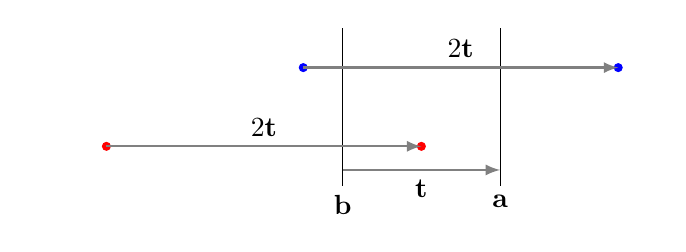
\begin{tikzpicture}
                % planes
                \draw (0,-1) node[below]{$\mathbf{b}$} -- (0,1) ;
                \draw (2,-1) node[below]{$\mathbf{a}$} -- (2,1) ;
                % intial points
                \draw[blue,fill=blue] (-0.5,0.5) circle (0.05);
                \draw[red,fill=red]  (-3,-0.5) circle (0.05);
                % second reflexion
                \draw[blue,fill=blue] (3.5,0.5) circle (0.05);
                \draw[red,fill=red]  (1,-0.5) circle (0.05);
                % line
                \draw[gray,thick,->,>=latex] (-0.5,0.5) -- node[midway,above,black]{$2\mathbf{t}$} (3.5,0.5);
                \draw[gray,thick,->,>=latex] (-3,-0.5)  -- node[midway,above,black]{$2\mathbf{t}$} (1,-0.5);
                %translation
                \draw[gray,thick,->,>=latex] (0,-0.8) -- node[midway,below,black]{$\mathbf{t}$} (2,-0.8);
                % clip
                \clip (-4,1) rectangle (4,1);
            \end{tikzpicture}
        }%
        \only<5>{%
            \begin{tikzpicture}
                % planes
                \draw[white] (0,-1) node[below]{$\mathbf{b}$} -- (0,1) ;
                \draw[white] (2,-1) node[below]{$\mathbf{a}$} -- (2,1) ;
                % intial points
                \draw[blue,fill=blue] (-0.5,0.5) circle (0.05);
                \draw[red,fill=red]  (-3,-0.5) circle (0.05);
                % second reflexion
                \draw[blue,fill=blue] (3.5,0.5) circle (0.05);
                \draw[red,fill=red]  (1,-0.5) circle (0.05);
                % line
                0\draw[gray,thick,->,>=latex] (-0.5,0.5) -- node[midway,above,black]{$2\mathbf{t}$} (3.5,0.5);
                \draw[gray,thick,->,>=latex] (-3,-0.5)  -- node[midway,above,black]{$2\mathbf{t}$} (1,-0.5);
                % clip
                \clip (-4,1) rectangle (4,1);
            \end{tikzpicture}
        }%
    \end{center}
    %\textbf{Double reflection:}
    %\begin{itemize}
    %\item $\mathbf{T}=\mathbf{ab} = 1 + \displaystyle\frac{t}{2}\mathbf{P}$
    %\item $\mathbf{X}'=\mathbf{ab} \mathbf{X} (\mathbf{ab})^{-1} = \mathbf{T} \mathbf{X} \mathbf{\widetilde{T}}$
    %\item $\mathbf{P} \rightarrow$ point at infinity $\Rightarrow \mathbf{P}^2=0$ 
    %\end{itemize}
\end{frame}



\begin{frame}{But in 3D?}
\end{frame}


%%%%%%%%%%%%%%%%%%%
\begin{frame}{Interpretation}
    \begin{center}
        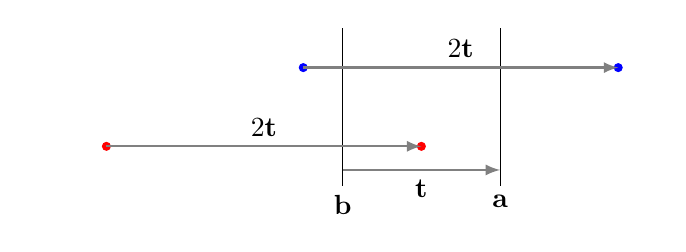
\begin{tikzpicture}
            % planes
            \draw (0,-1) node[below]{$\mathbf{b}$} -- (0,1) ;
            \draw (2,-1) node[below]{$\mathbf{a}$} -- (2,1) ;
            % intial points
            \draw[blue,fill=blue] (-0.5,0.5) circle (0.05);
            \draw[red,fill=red]  (-3,-0.5) circle (0.05);
            % second reflexion
            \draw[blue,fill=blue] (3.5,0.5) circle (0.05);
            \draw[red,fill=red]  (1,-0.5) circle (0.05);
            % line
            \draw[gray,thick,->,>=latex] (-0.5,0.5) -- node[midway,above,black]{$2\mathbf{t}$} (3.5,0.5);
            \draw[gray,thick,->,>=latex] (-3,-0.5)  -- node[midway,above,black]{$2\mathbf{t}$} (1,-0.5);
            %translation
            \draw[gray,thick,->,>=latex] (0,-0.8) -- node[midway,below,black]{$\mathbf{t}$} (2,-0.8);
            % clip
            \clip (-4,1) rectangle (4,1);
        \end{tikzpicture}
    \end{center}
    \begin{itemize}
        \item any combinaison of 2 successive reflexions $\leftrightarrow$ combinaison of rotation / translation \\
              $\hookrightarrow$ rigid transformation
        \item quaternions and dual quaternions are a special form of motors, in 3D.
        \item motors (double reflexion) works in any dimension !
    \end{itemize}
\end{frame}



%%%%%%%%%%%%%%%%%%
\begin{frame}{Reflexions are generic}
    $$ \mathbf{a}\Big( \textcolor{blue}{\mathbf{x} \wedge \mathbf{y} \wedge  ... \wedge \mathbf{z}} \Big) \mathbf{a}^{-1}
        = (\mathbf{a}\textcolor{blue}{\mathbf{x}} \mathbf{a}^{-1}) \wedge (\mathbf{a}\textcolor{blue}{\mathbf{y}} \mathbf{a}^{-1}) \wedge  ... \wedge  (\mathbf{a}\textcolor{blue}{\mathbf{z}} \mathbf{a}^{-1})$$
    ~\\
    \textbf{Same versor for any object:}
    $$
        \mathbf{a}
        \left\lbrace
        \begin{array}{c}
            \text{point} \\
            \text{line}  \\
            \text{plane} \\
            \vdots
        \end{array}
        \right\rbrace
        \mathbf{a}^{-1}
    $$
\end{frame}






%%%%%%%%%%%%%%%%%%%%%%%%%%%%%%%%%%%%%%%%%%%%%%%%%%%%%%%%%%%%%%%%%%%%%%%
\section{Demo}

%%%%%%%%%%%%%%%%
\begin{frame}{Demo in Python}
    \hfill\href{https://tbuli.github.io/teahouse/lab/index.html}{\beamergotobutton{a cube and a string}}
\end{frame}


\begin{frame}{Geometric algebra}
    conclusion
\end{frame}



\end{document}


